% small.tex
\documentclass{beamer}
%\usetheme{default}
\usetheme{Warsaw}
\usecolortheme{whale}
\usepackage{tikz}
\usepackage[absolute,overlay]{textpos}
\usepackage{soul}
\usepackage{pdfpages}
\usepackage[most]{tcolorbox}
%\usepackage{multirow}
\usepackage{tikz,amsmath,array}
\usepackage{hyperref}

\newcommand{\greekbf}[1]{\boldsymbol{\mathrm{#1}}}
\newcommand{\btVFill}{\vskip0pt plus 1filll}
\newcolumntype{P}[1]{>{\centering\arraybackslash}p{#1}}

%\setbeamertemplate{background}[grid][step=.25\textwidth]

\title[Bayesian Statistics]{Bayesian Statistics Guest Lecture}
%\subtitle
\author{Michael Holton Price}
\institute[SFI] {
	Santa Fe Institute\\
	MichaelHoltonPrice@gmail.com\\
	\line(1,0){0}\\
	Penn State: Anthro 508\\
	06 Apr 2021\\
}
%\date{05 Feb 2014}
\date{}

% Note: default dimensions are 128 mm by 96 mm (4 x 3)
\begin{document}

%----------- titlepage ----------------------------------------------%
\begin{frame}[plain]
  \titlepage
\end{frame}

%----------- slide --------------------------------------------------%
\begin{frame}[t]
  \frametitle{I have things to go over, but I'm as happy to just have a virtual whiteboard session}
\end{frame}

%----------- slide --------------------------------------------------%
\begin{frame}[t]
  \frametitle{If you're confused by probability notation... you should be!}
  \begin{minipage}{0\linewidth}
\begin{flushleft}
\begin{equation*}
  \mbox{Probability for the variable A:}
\end{equation*}
\begin{equation*}
  P(A)
\end{equation*}
\pause
\begin{equation*}
  \mbox{Probability for the variable P:}
\end{equation*}
\begin{equation*}
  P(B)
\end{equation*}
\pause
\begin{equation*}
  \mbox{P is not the same object, but it has the same symbol.}
\end{equation*}
\begin{equation*}
  \mbox{Mathematicians sometimes call this abuse of notation.}
\end{equation*}
\end{flushleft} 
\end{minipage}
\end{frame}

%----------- slide --------------------------------------------------%
\begin{frame}[t]
  \frametitle{There are random variables and realizations of those random variables}
  \begin{minipage}{0\linewidth}
\begin{flushleft}
\begin{equation*}
  \mbox{A is the random variable and a is a realization:}
\end{equation*}
\begin{equation*}
  P_A(A=a)
\end{equation*}
\pause
\begin{equation*}
  P_B(B=b)
\end{equation*}
\pause
\begin{equation*}
  \mbox{Careful use of notation gets awkward fast.}
\end{equation*}
\pause
\begin{equation*}
  \mbox{I will be abusing notation.}
\end{equation*}
\pause
\begin{equation*}
  \mbox{You deserve to know people have been doing it to you all}
\end{equation*}
\begin{equation*}
  \mbox{the time without telling you.}
\end{equation*}
\end{flushleft} 
\end{minipage}
\end{frame}

%----------- slide --------------------------------------------------%
\begin{frame}[t]
  \frametitle{Bayes' theorem is intuitive}
  \begin{minipage}{0\linewidth}
\begin{flushleft}
\begin{equation*}
  \mbox{The joint probability of A and B:}
\end{equation*}
\begin{equation*}
  p(A,B)
\end{equation*}
\pause
\begin{equation*}
  \mbox{Introducing the conditional probability:}
\end{equation*}
\begin{equation*}
  p(A,B) = p(A|B) p(B)
\end{equation*}
\pause
\begin{equation*}
  p(A,B) = p(B|A) p(A)
\end{equation*}
\pause
\begin{equation*}
  p(A|B) = \frac{p(B|A) p(A)}{p(B)}
\end{equation*}
\end{flushleft} 
\end{minipage}
\end{frame}

%----------- slide --------------------------------------------------%
\begin{frame}[t]
  \frametitle{Bayes' theorem is intuitive}
  \begin{minipage}{0\linewidth}
\begin{flushleft}
\begin{equation*}
  p(A|B) = \frac{p(B|A) p(A)}{p(B)}
\end{equation*}
\pause
\begin{equation*}
  p(\theta|D) = \frac{p(D|\theta) p(\theta)}{p(D)}
\end{equation*}
\pause
\begin{equation*}
  p(\theta|D,\alpha) = \frac{p(D|\theta) p(\theta|\alpha)}{p(D)}
\end{equation*}

\end{flushleft} 
\end{minipage}
\end{frame}

%----------- slide --------------------------------------------------%
\begin{frame}
  \frametitle{Bayesian demographic inference}
  \begin{center}
	\begin{equation*}
          p(\greekbf{\theta}|\mathbf{D},\greekbf{\alpha}) = \frac{p(\mathbf{D}|\greekbf{\theta}) \, p(\greekbf{\theta}|\greekbf{\alpha})}{p(\mathbf{D}|\greekbf{\alpha})}
        \end{equation*}
  \end{center}

  \pause
  \begin{center}
          \begin{equation*}
            \begin{array}{lll}
	      \greekbf{\alpha} & := & \mbox{Hyperparameter specifying priors}\\
                               &    &\\
              \greekbf{\theta} & := & \mbox{Parameter for demographic models}\\
	      \pause
                               &    &\\
              \mathbf{D}       & := & \mbox{Data}\\
                               &    &\\
            \end{array}
          \end{equation*}
  \end{center}
\end{frame}

%----------- slide --------------------------------------------------%
\begin{frame}[t]
    \frametitle{Bayesian Inference}
    \begin{columns}[c]
        \column{.333\textwidth}
            \begin{flushright}
                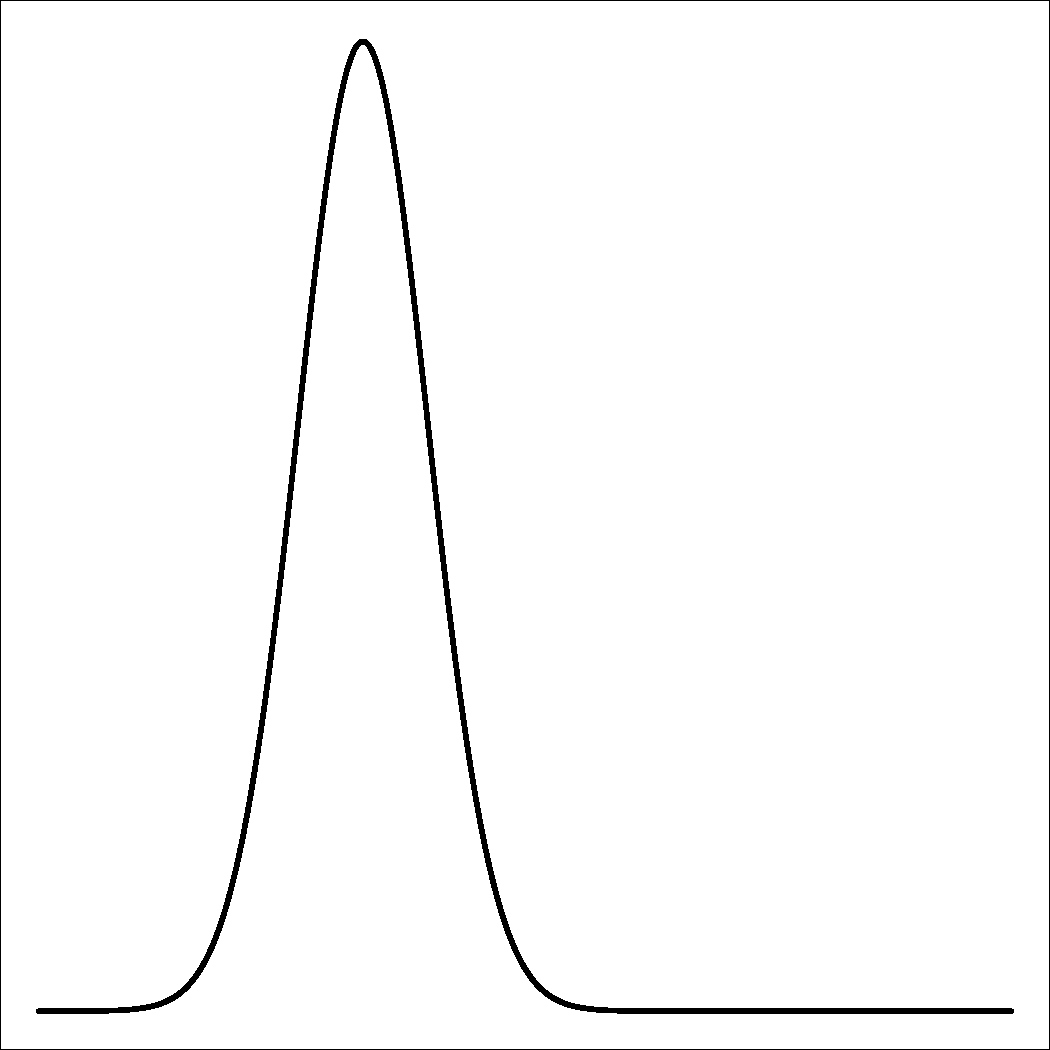
\includegraphics[width=1\textwidth]{bayesian_update_illustration_th1.pdf}
            \end{flushright}
        \column{.333\textwidth}
            \begin{flushright}
                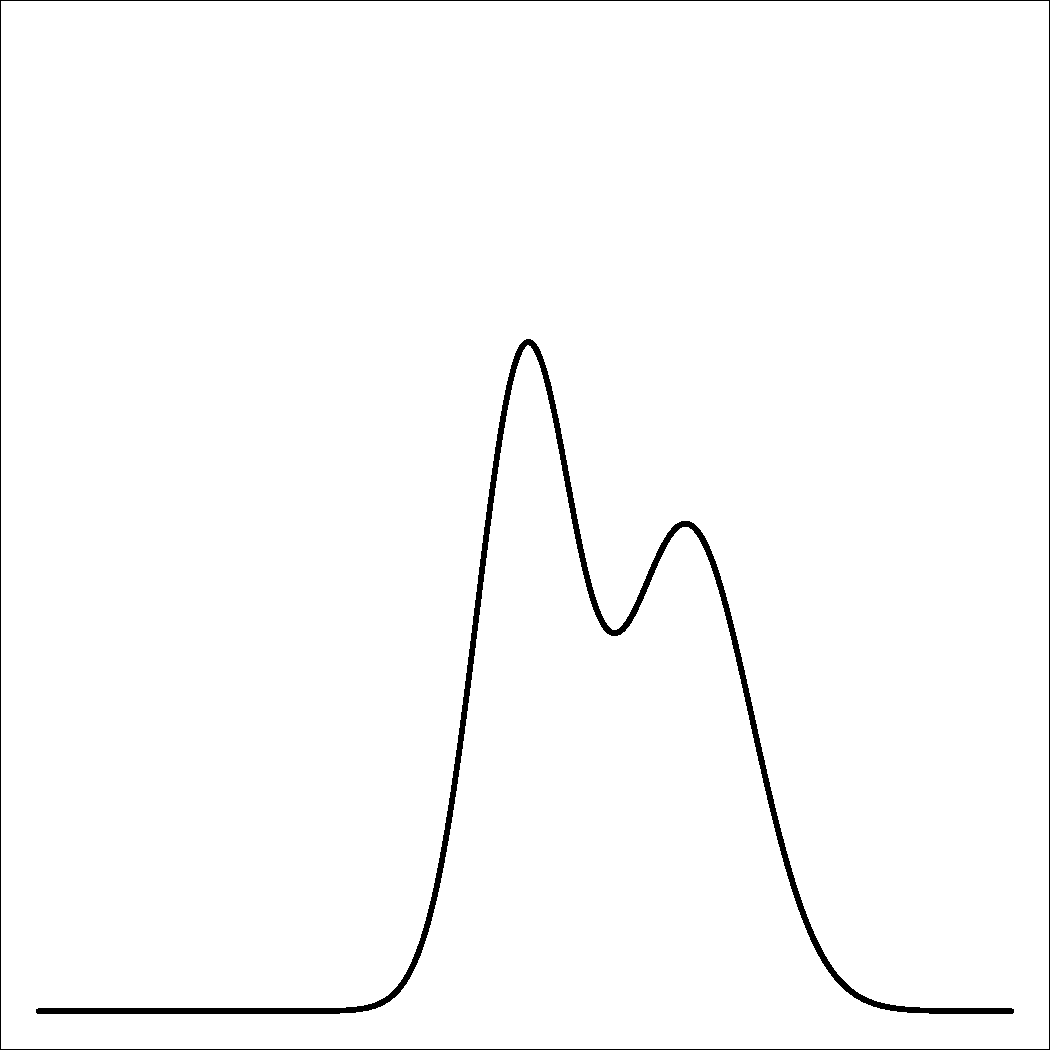
\includegraphics[width=1\textwidth]{bayesian_update_illustration_th2.pdf}
            \end{flushright}
        \column{.333\textwidth}
            \begin{flushright}
                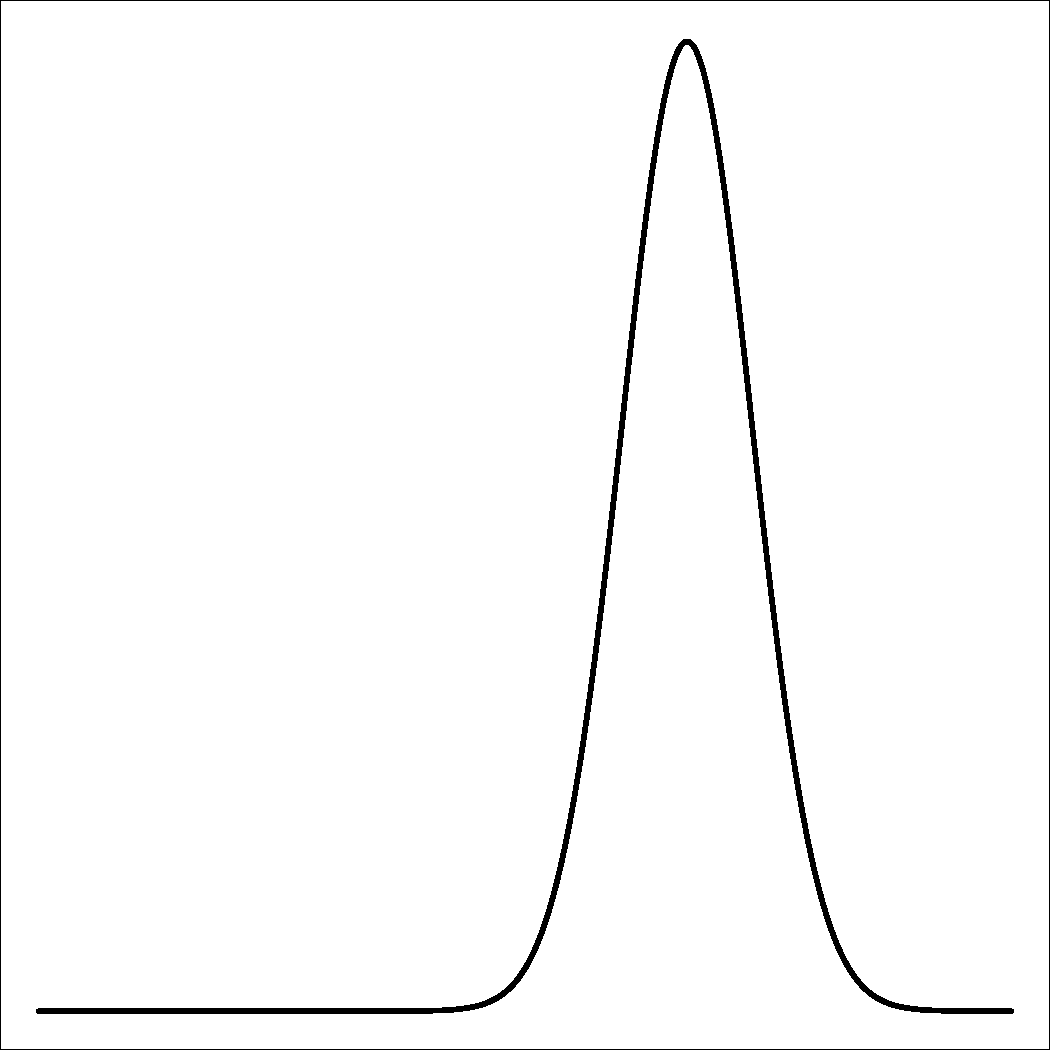
\includegraphics[width=1\textwidth]{bayesian_update_illustration_th3.pdf}
            \end{flushright}
    \end{columns}
\end{frame}

%----------- slide --------------------------------------------------%
\begin{frame}[t]
    \frametitle{Bayesian Inference}
    \begin{columns}[c]
        \column{.333\textwidth}
            \begin{flushright}
                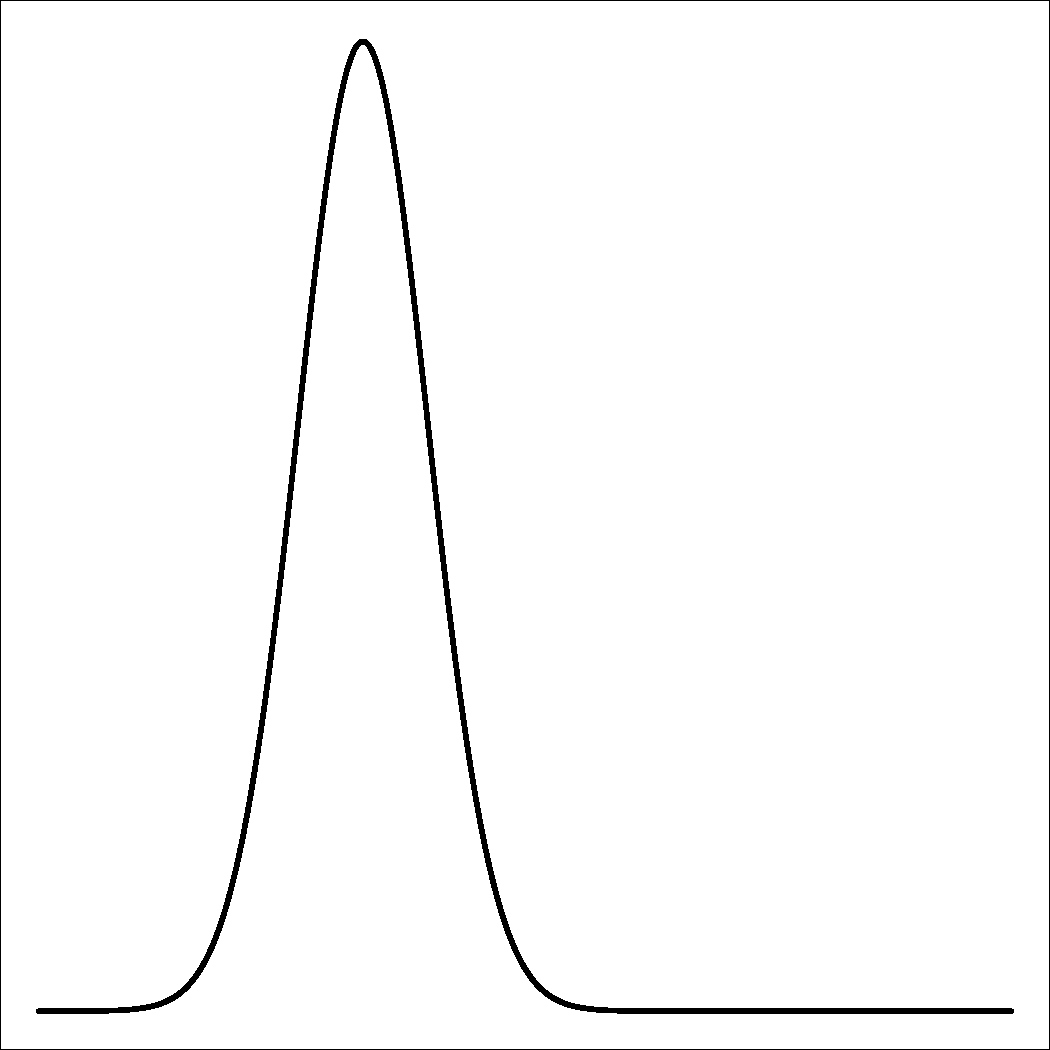
\includegraphics[width=1\textwidth]{bayesian_update_illustration_th1.pdf}\\
                \vspace{10pt}
                \Large Prior \hfill $0.40$\\
            \end{flushright}
        \column{.333\textwidth}
            \begin{flushright}
                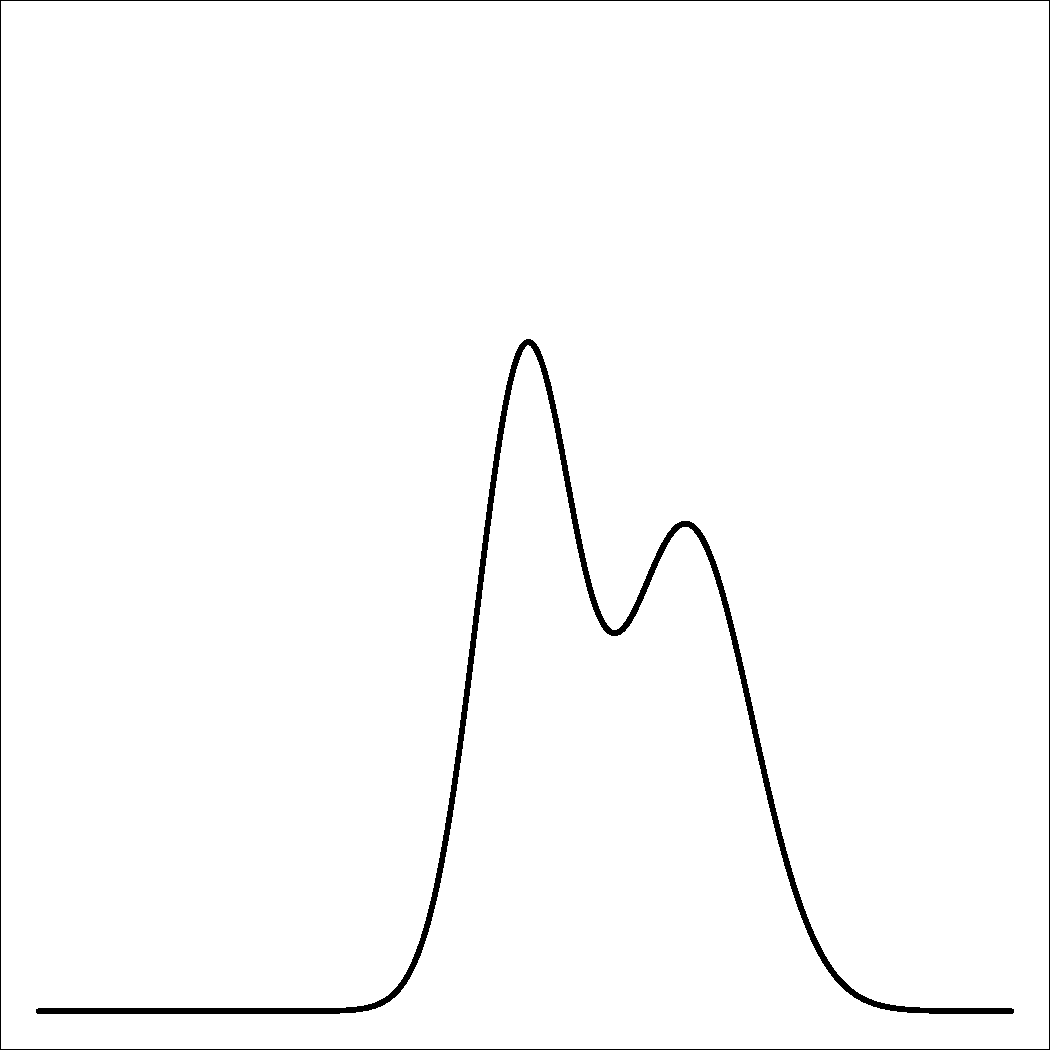
\includegraphics[width=1\textwidth]{bayesian_update_illustration_th2.pdf}\\
                \vspace{10pt}
                \Large $0.20$\\
            \end{flushright}
        \column{.333\textwidth}
            \begin{flushright}
                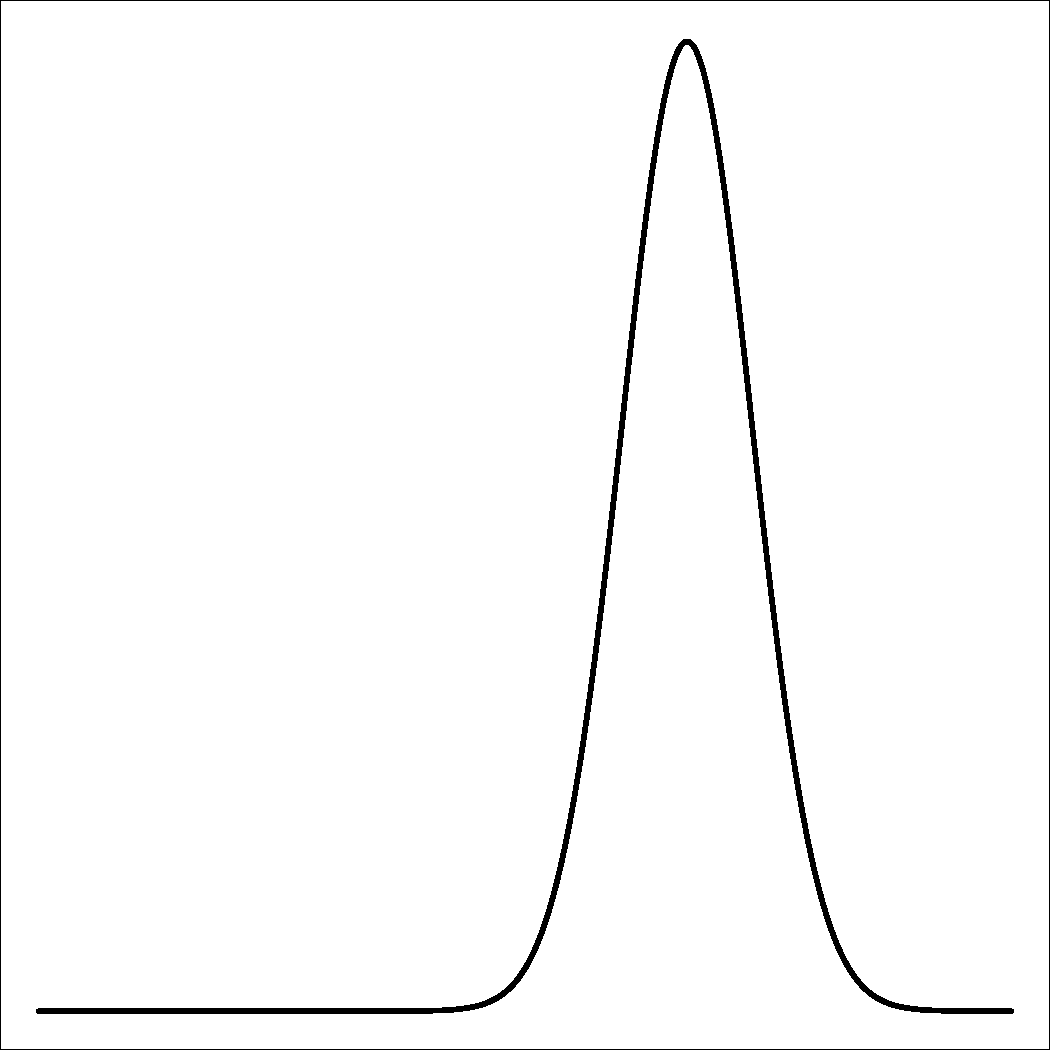
\includegraphics[width=1\textwidth]{bayesian_update_illustration_th3.pdf}\\
                \vspace{10pt}
                \Large $0.4$\\
            \end{flushright}
    \end{columns}
\end{frame}

%----------- slide --------------------------------------------------%
\begin{frame}[t]
    \frametitle{Bayesian Inference}
    \begin{columns}[c]
        \column{.333\textwidth}
            \begin{flushright}
                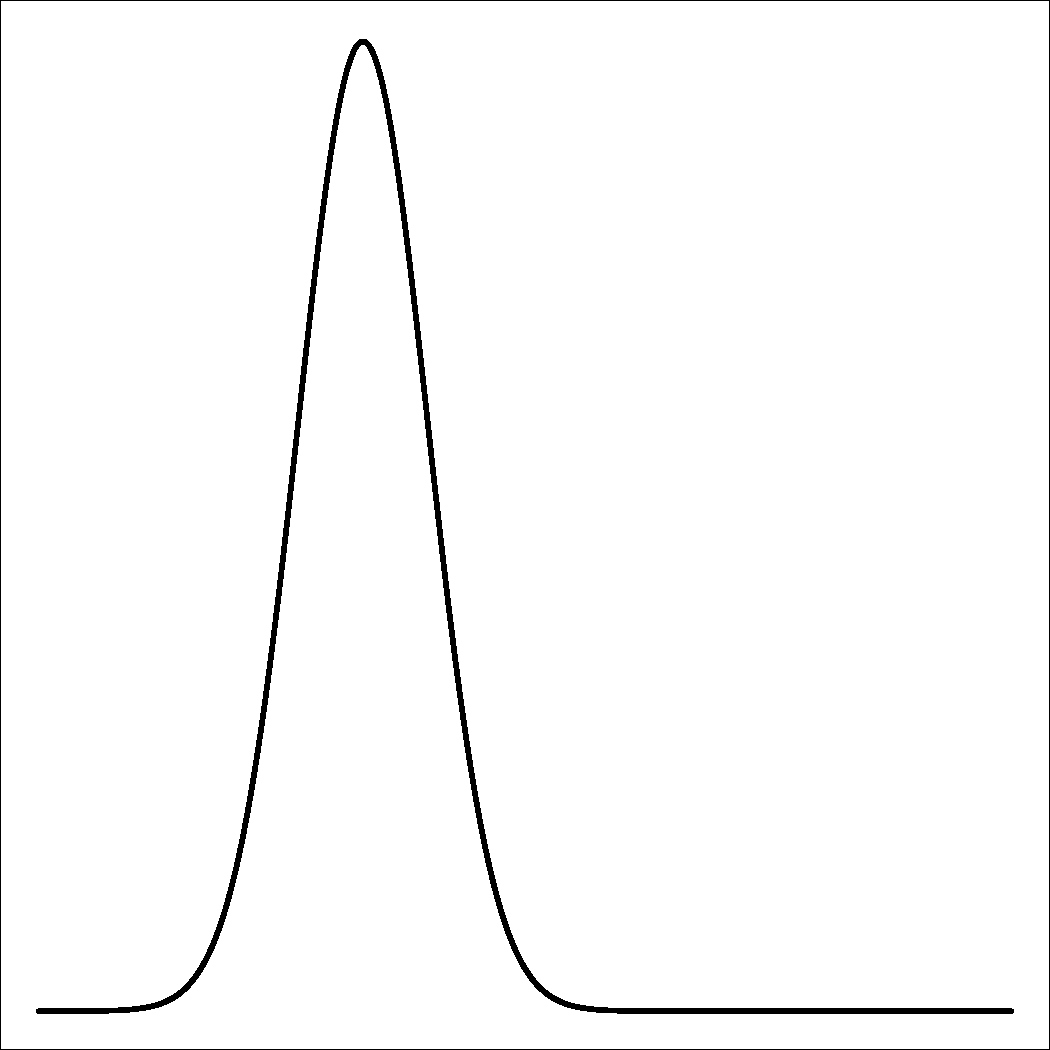
\includegraphics[width=1\textwidth]{bayesian_update_illustration_th1.pdf}\\
                \vspace{10pt}
                \Large Prior \hfill $0.40$\\
                \vspace{20pt}
                \Large Likelihood \hfill $0.02$\\
            \end{flushright}
        \column{.333\textwidth}
            \begin{flushright}
                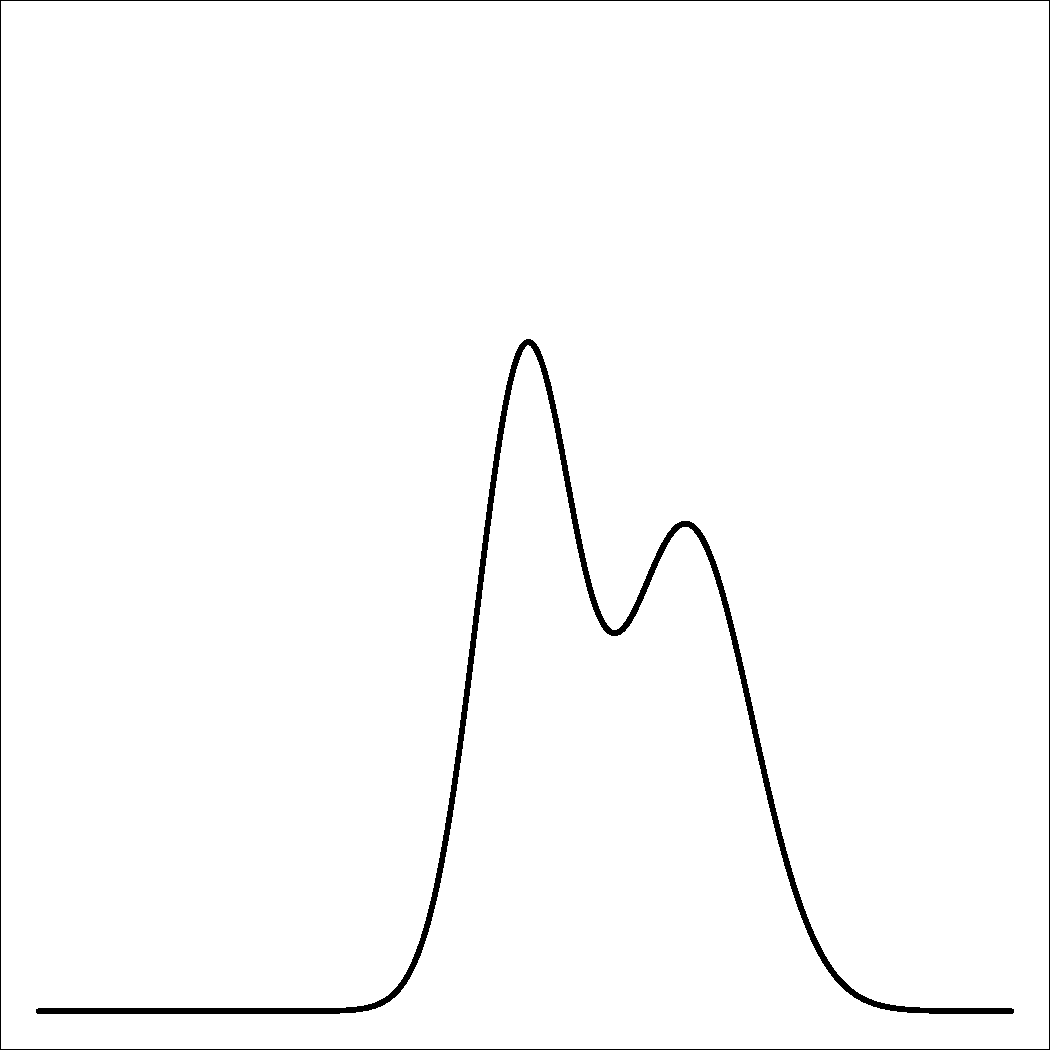
\includegraphics[width=1\textwidth]{bayesian_update_illustration_th2.pdf}\\
                \vspace{10pt}
                \Large $0.20$\\
                \vspace{20pt}
                \Large $1.00$\\
            \end{flushright}
        \column{.333\textwidth}
            \begin{flushright}
                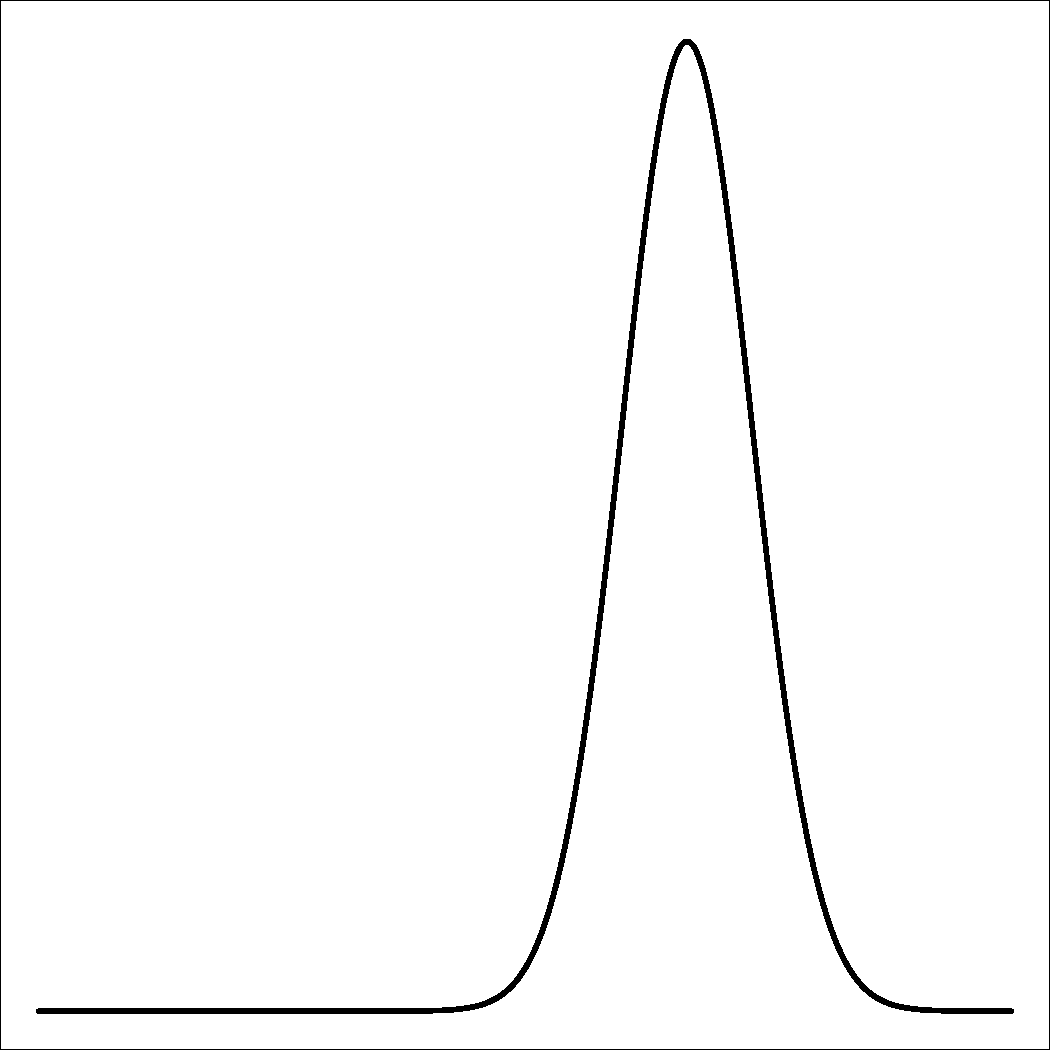
\includegraphics[width=1\textwidth]{bayesian_update_illustration_th3.pdf}\\
                \vspace{10pt}
                \Large $0.4$\\
                \vspace{20pt}
                \Large $0.04$\\
            \end{flushright}
    \end{columns}
\end{frame}

%----------- slide --------------------------------------------------%
\begin{frame}[t]
    \frametitle{Bayesian Inference}
    \begin{columns}[c]
        \column{.333\textwidth}
            \begin{flushright}
                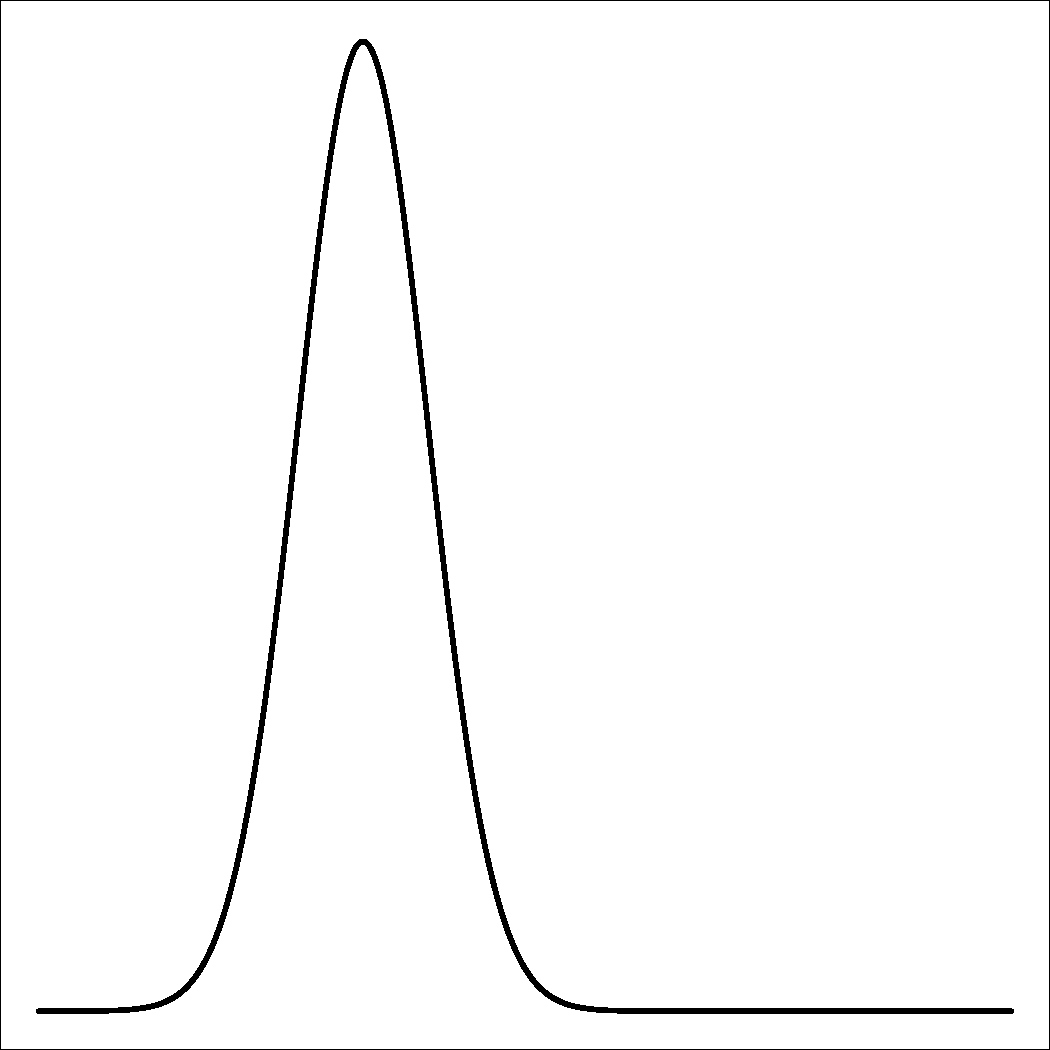
\includegraphics[width=1\textwidth]{bayesian_update_illustration_th1.pdf}\\
                \vspace{10pt}
                \Large Prior \hfill $0.40$\\
                \vspace{20pt}
                \Large Likelihood \hfill $0.02$\\
                \vspace{20pt}
                \Large Posterior \hfill $0.02$
            \end{flushright}
        \column{.333\textwidth}
            \begin{flushright}
                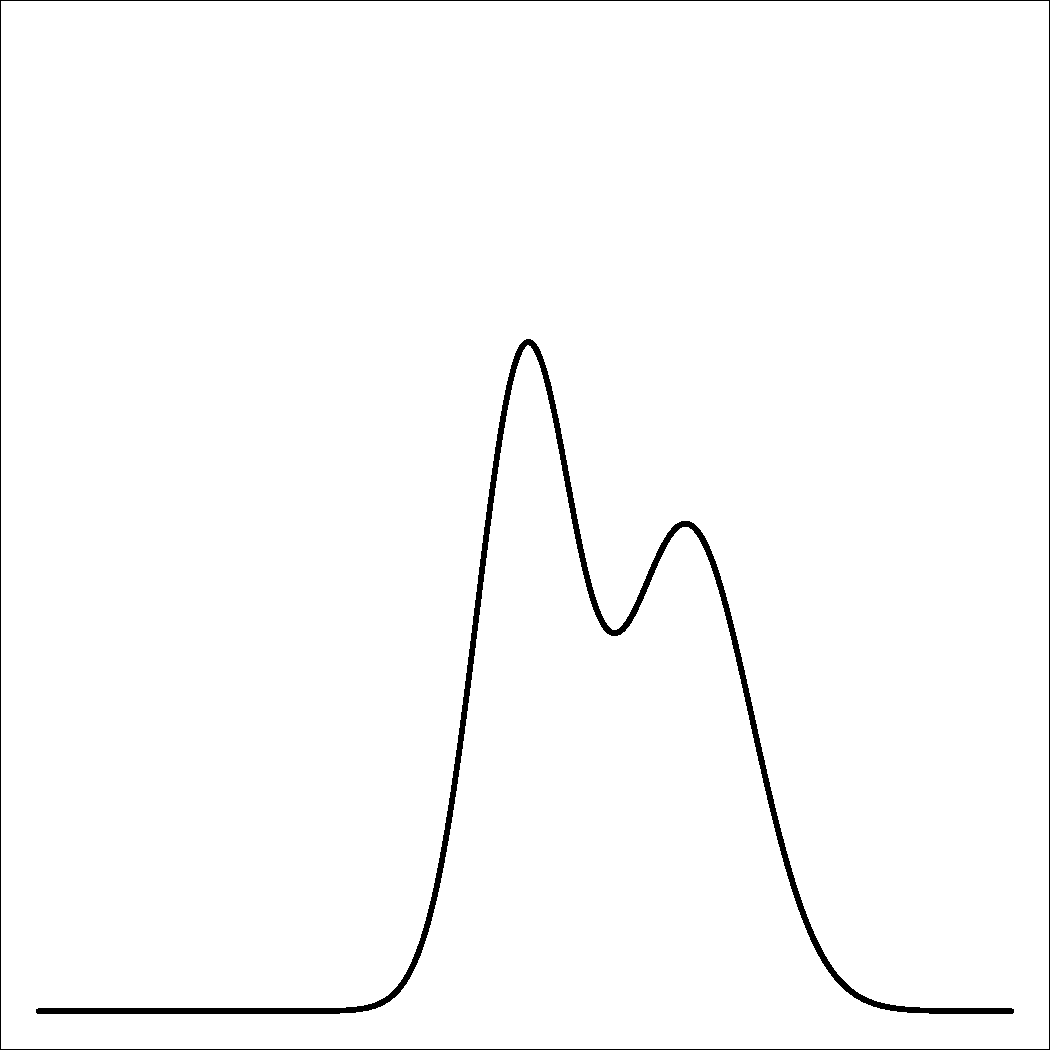
\includegraphics[width=1\textwidth]{bayesian_update_illustration_th2.pdf}\\
                \vspace{10pt}
                \Large $0.20$\\
                \vspace{20pt}
                \Large $1.00$\\
                \vspace{20pt}
                \Large $0.94$
            \end{flushright}
        \column{.333\textwidth}
            \begin{flushright}
                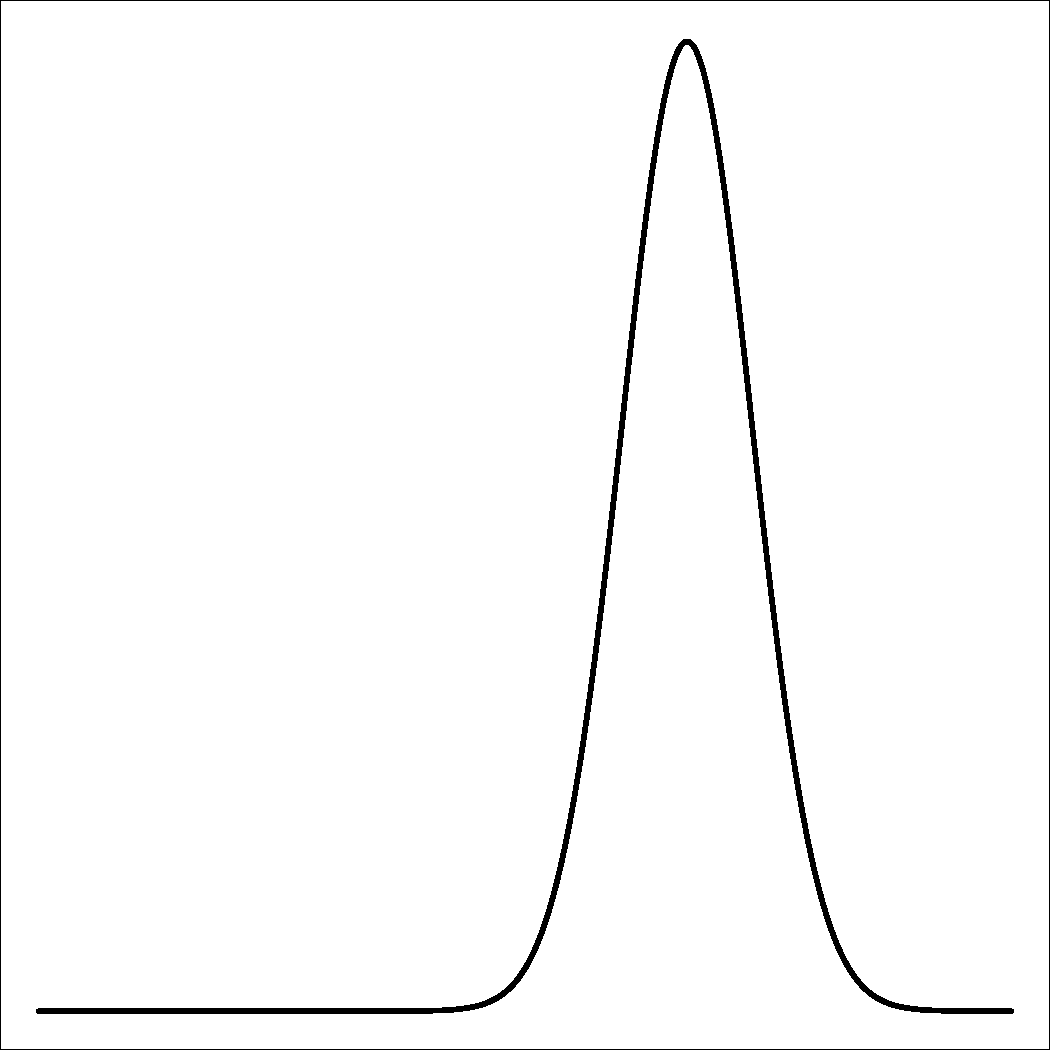
\includegraphics[width=1\textwidth]{bayesian_update_illustration_th3.pdf}\\
                \vspace{10pt}
                \Large $0.4$\\
                \vspace{20pt}
                \Large $0.04$\\
                \vspace{20pt}
                \Large $0.04$
            \end{flushright}
    \end{columns}
\end{frame}

%----------- slide --------------------------------------------------%
\begin{frame}[t]
    \frametitle{Bayesian Inference}
    \begin{columns}[c]
        \column{.333\textwidth}
            \begin{flushright}
                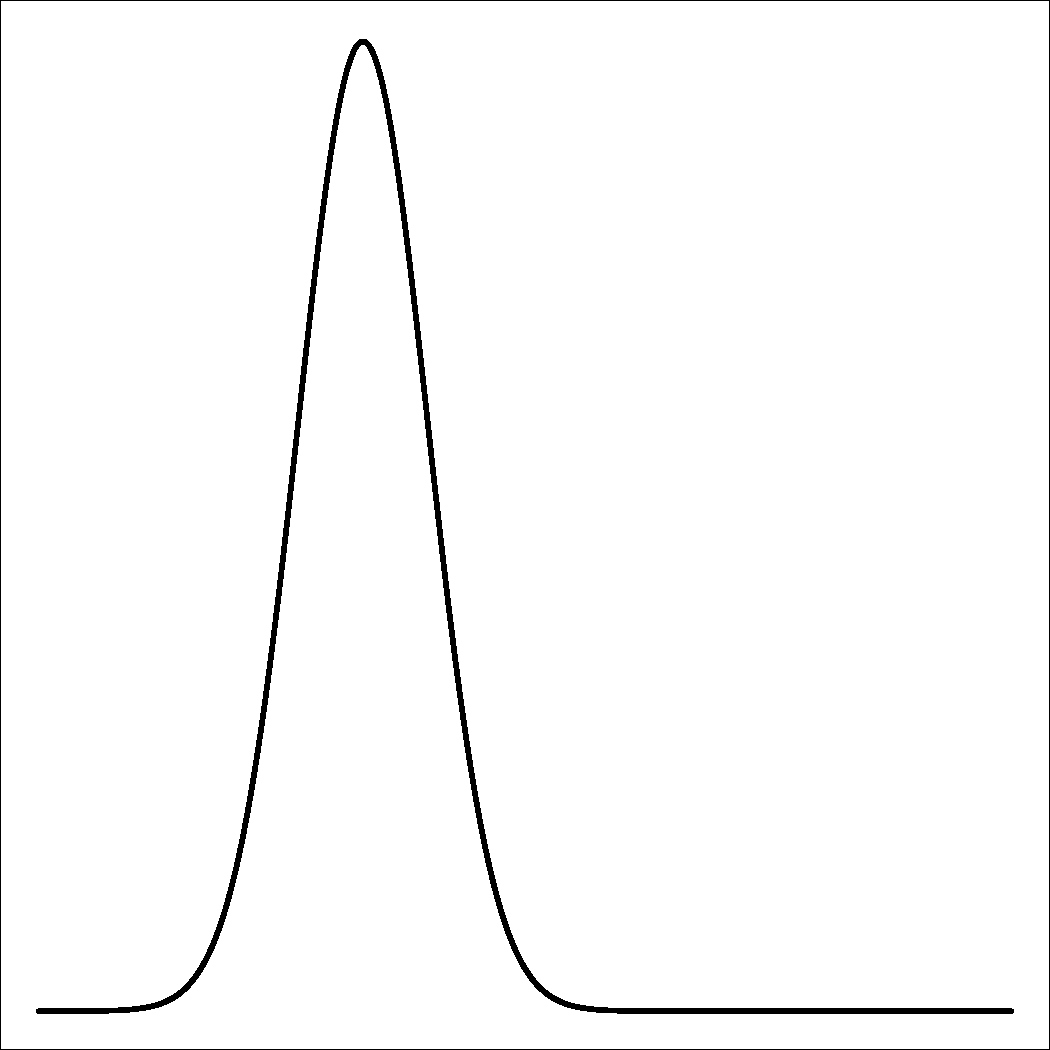
\includegraphics[width=1\textwidth]{bayesian_update_illustration_th1.pdf}\\
                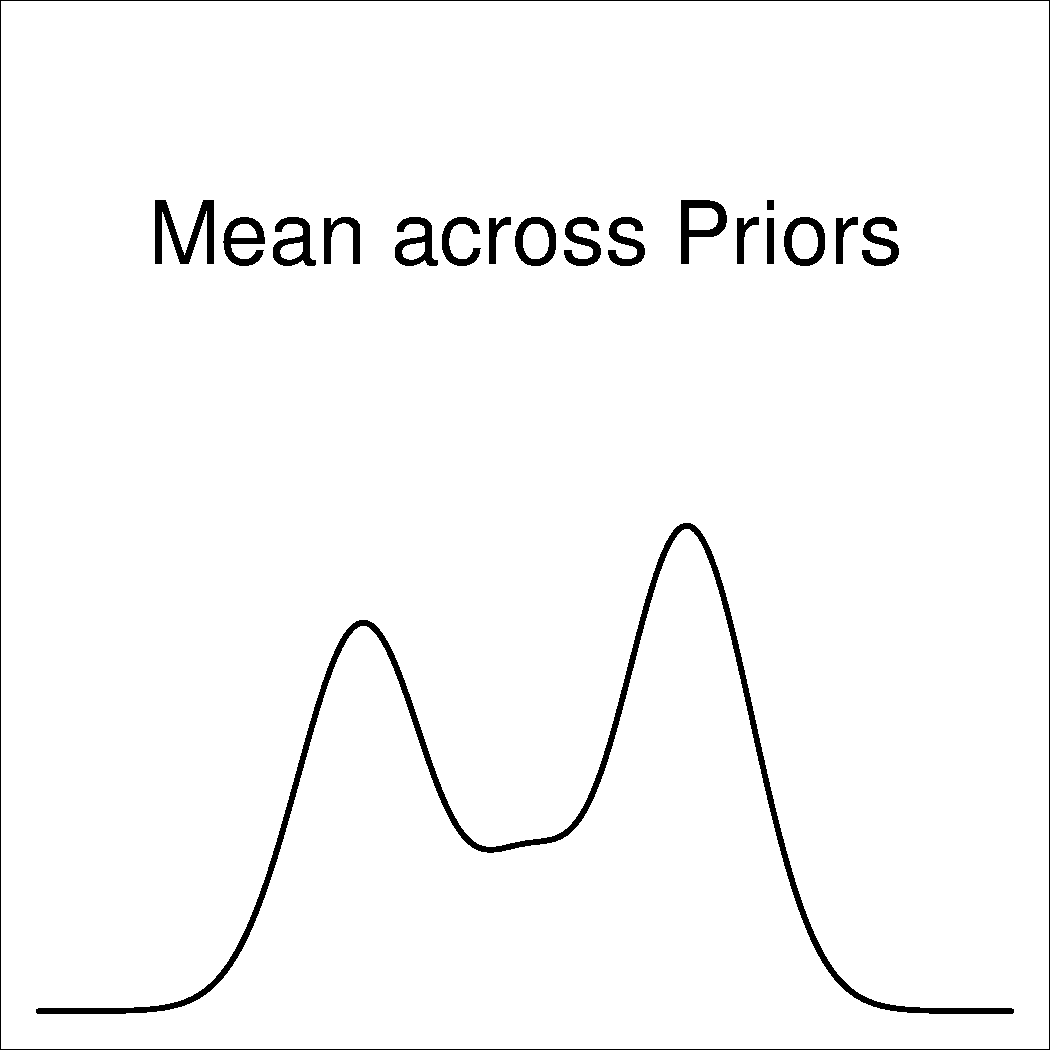
\includegraphics[width=1\textwidth]{bayesian_update_illustration_prior.pdf}\\
            \end{flushright}
        \column{.333\textwidth}
            \begin{flushright}
                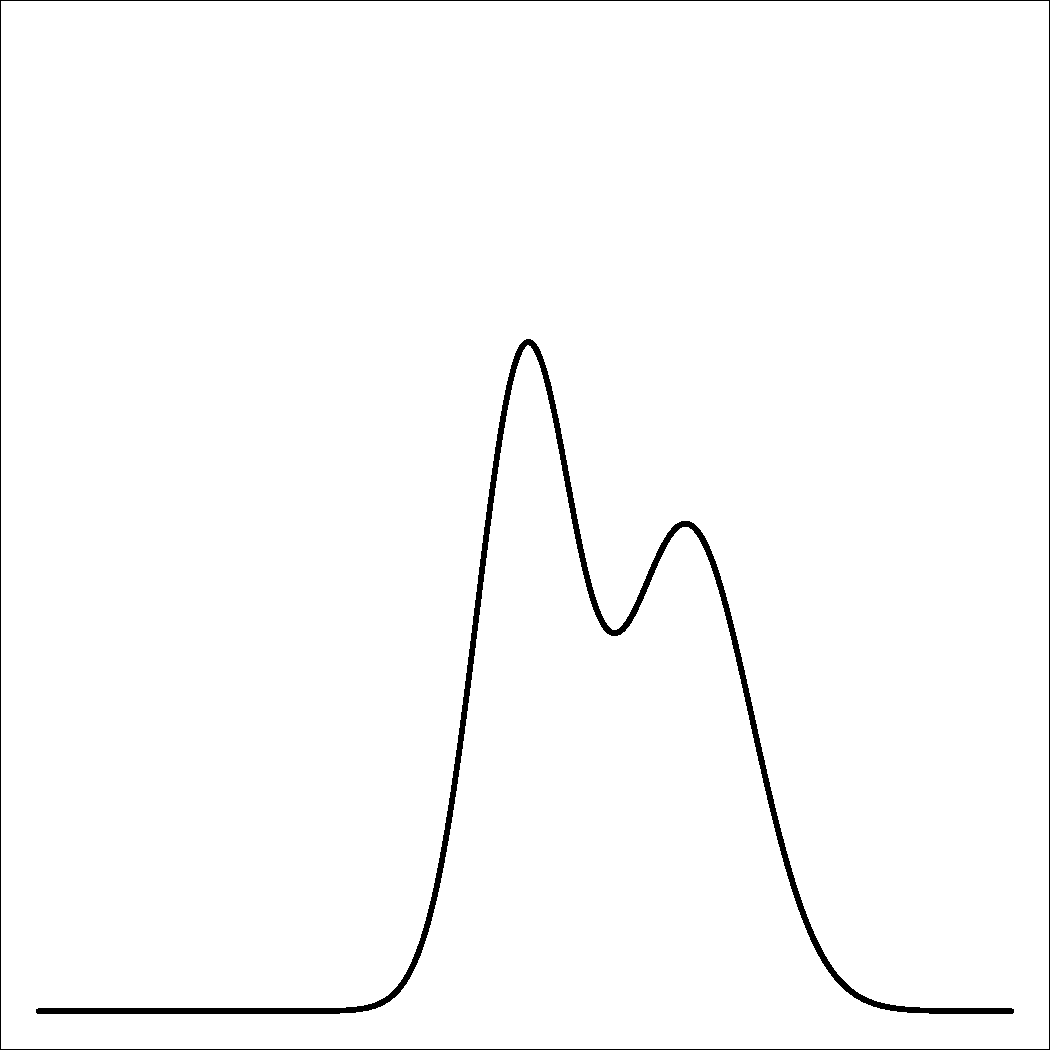
\includegraphics[width=1\textwidth]{bayesian_update_illustration_th2.pdf}\\
                
\includegraphics[width=1\textwidth]{bayesian_update_illustration_blank.pdf}\\
            \end{flushright}
        \column{.333\textwidth}
            \begin{flushright}
                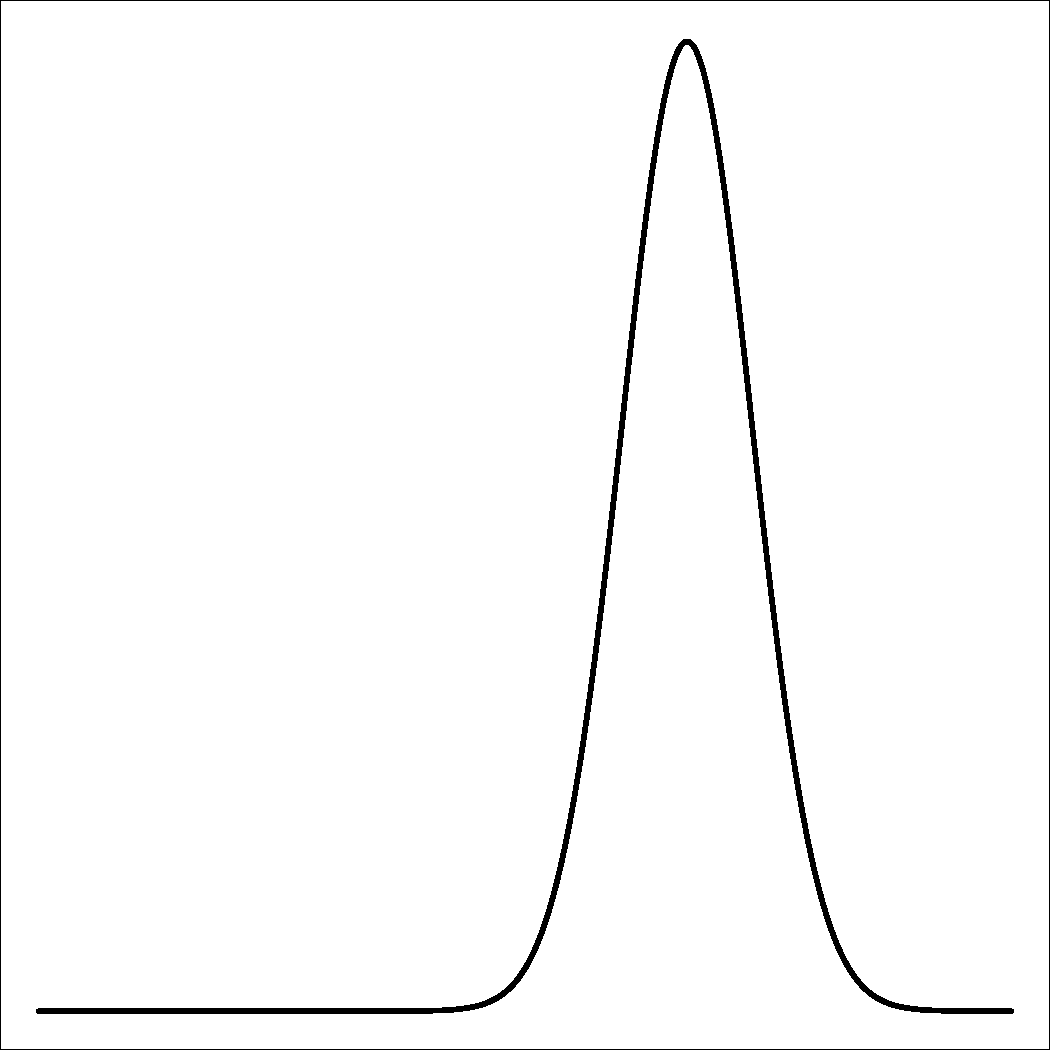
\includegraphics[width=1\textwidth]{bayesian_update_illustration_th3.pdf}\\
                
\includegraphics[width=1\textwidth]{bayesian_update_illustration_blank.pdf}\\
            \end{flushright}
    \end{columns}
\end{frame}

%----------- slide --------------------------------------------------%
\begin{frame}[t]
    \frametitle{Bayesian Inference}
    \begin{columns}[c]
        \column{.333\textwidth}
            \begin{flushright}
                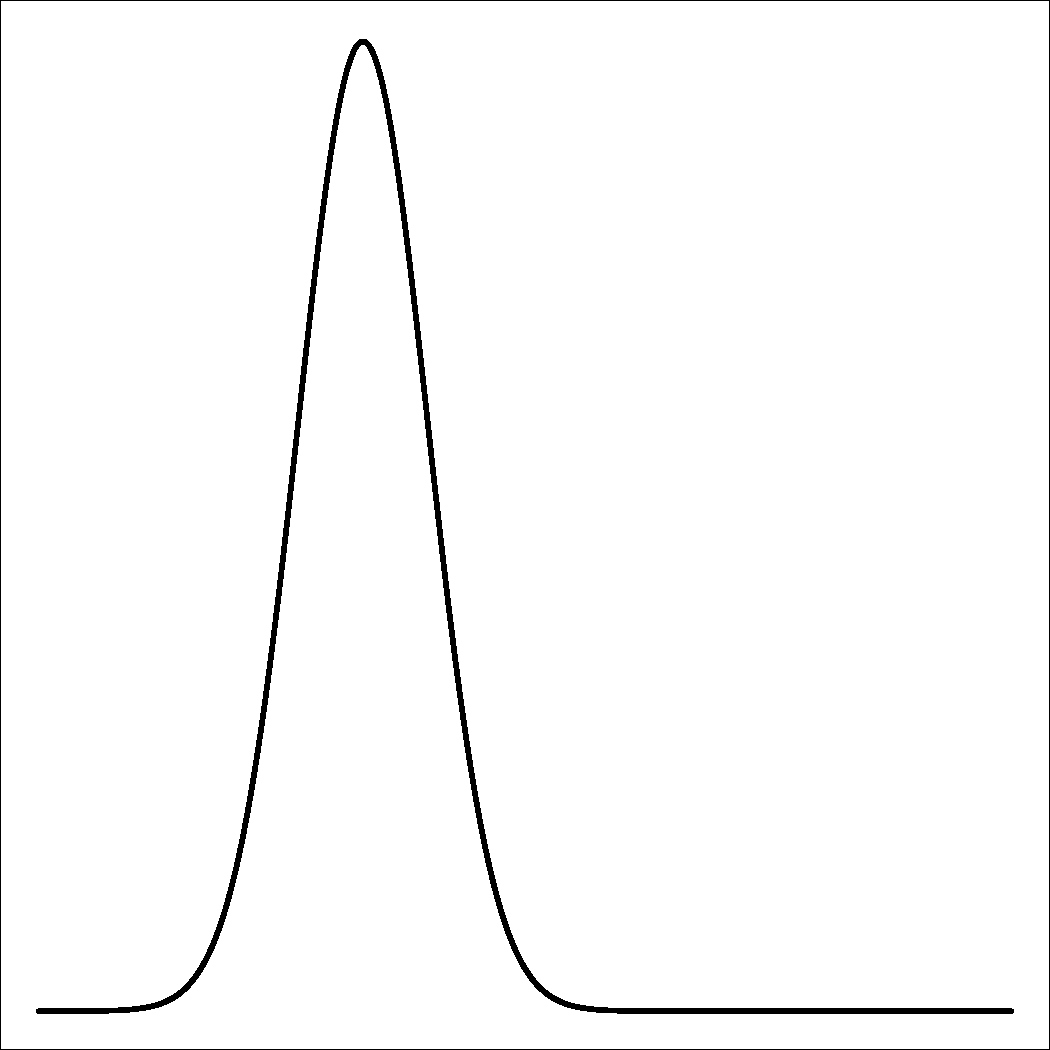
\includegraphics[width=1\textwidth]{bayesian_update_illustration_th1.pdf}\\
                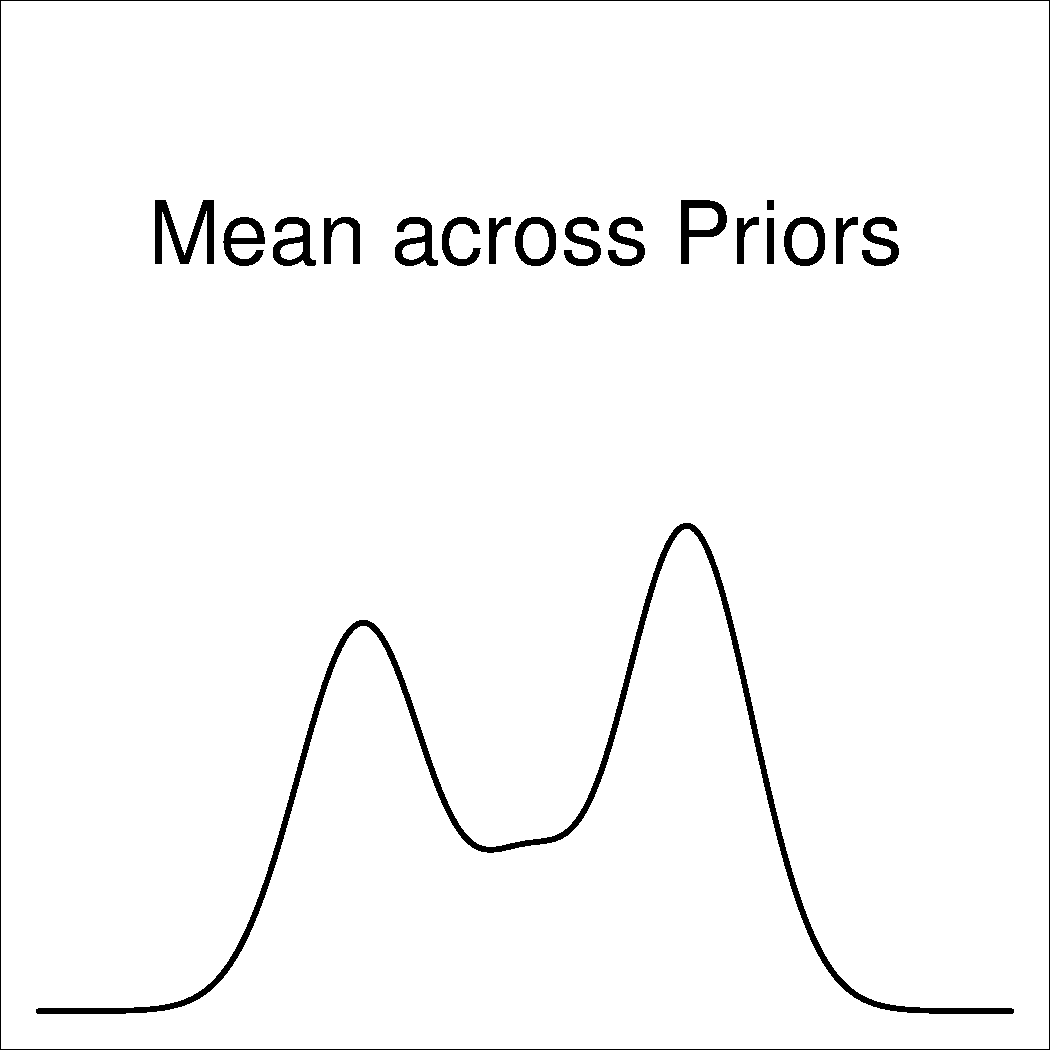
\includegraphics[width=1\textwidth]{bayesian_update_illustration_prior.pdf}\\
            \end{flushright}
        \column{.333\textwidth}
            \begin{flushright}
                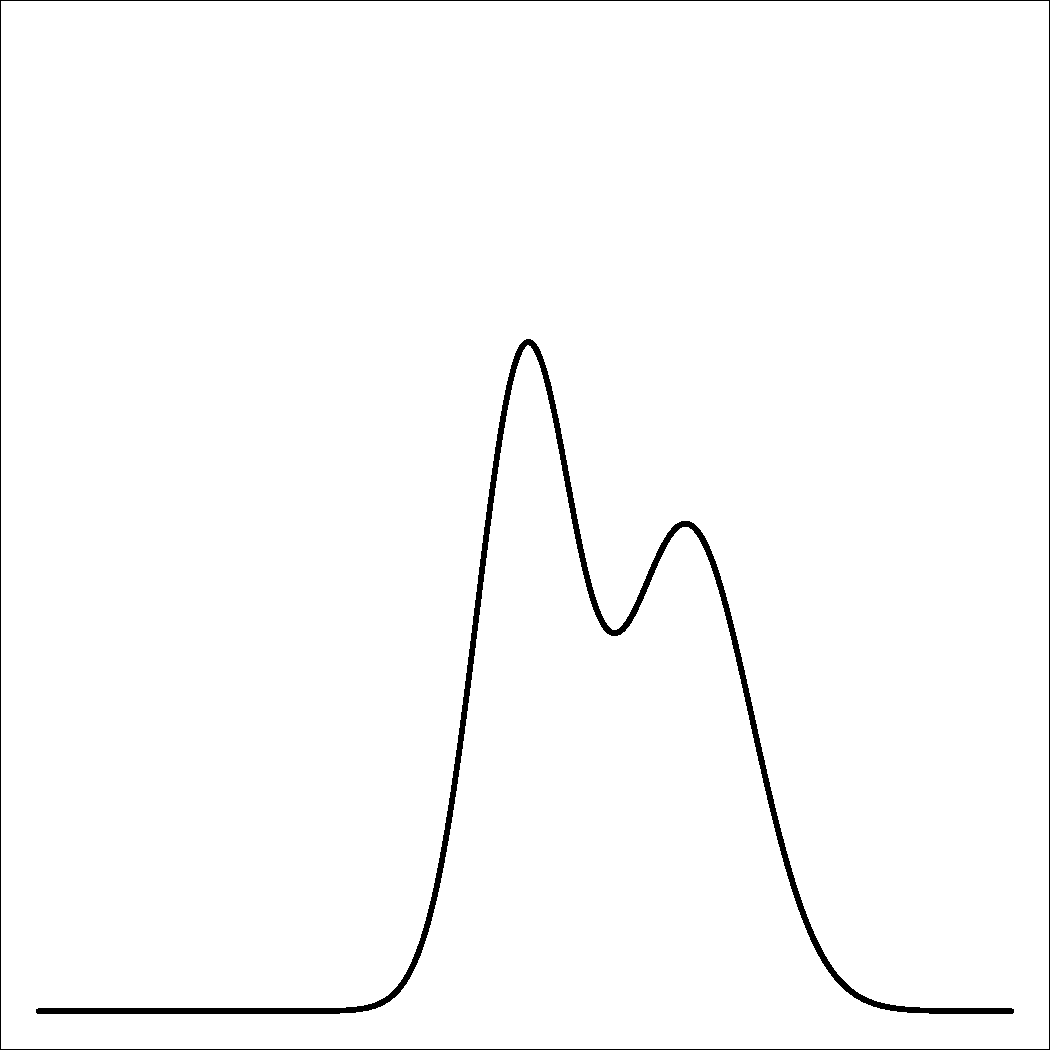
\includegraphics[width=1\textwidth]{bayesian_update_illustration_th2.pdf}\\
                
\includegraphics[width=1\textwidth]{bayesian_update_illustration_blank.pdf}\\
            \end{flushright}
        \column{.333\textwidth}
            \begin{flushright}
                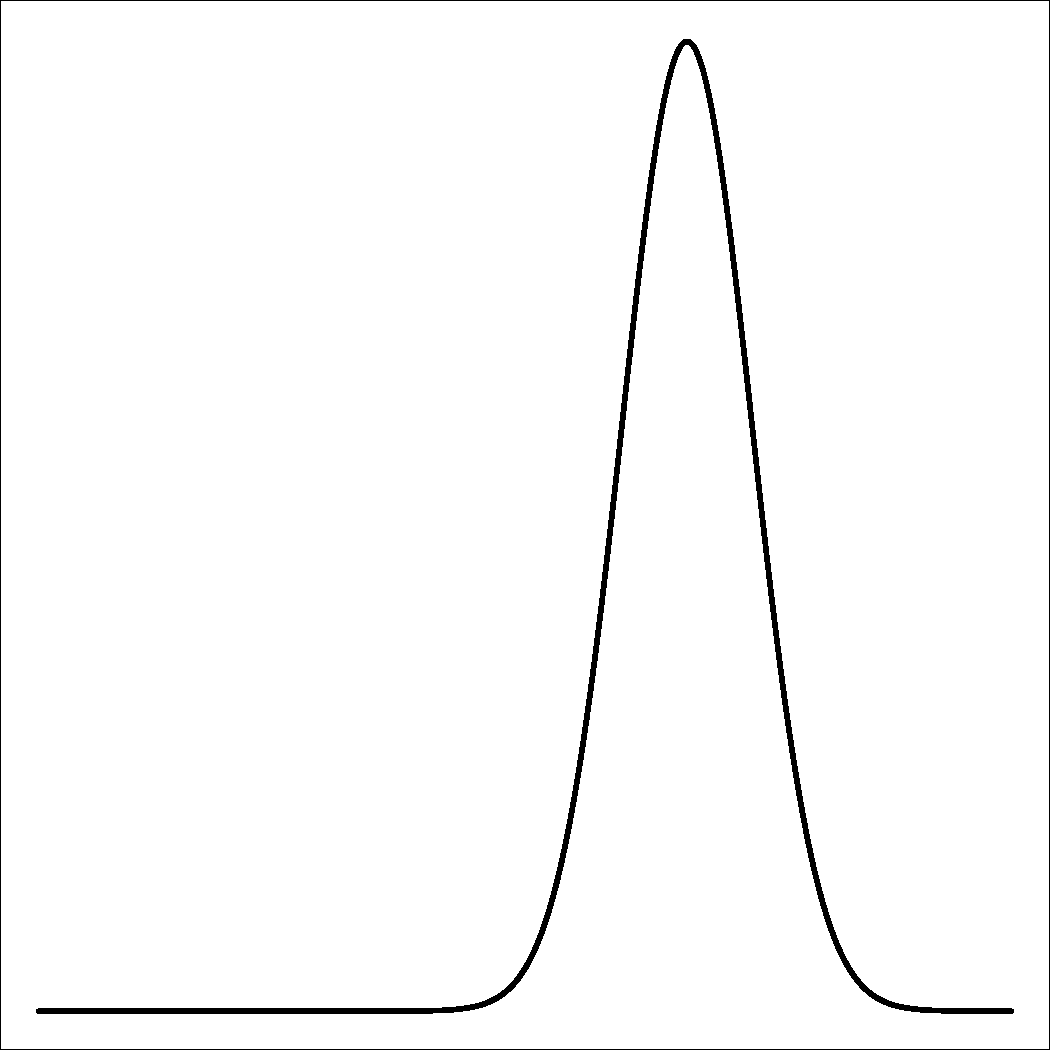
\includegraphics[width=1\textwidth]{bayesian_update_illustration_th3.pdf}\\
                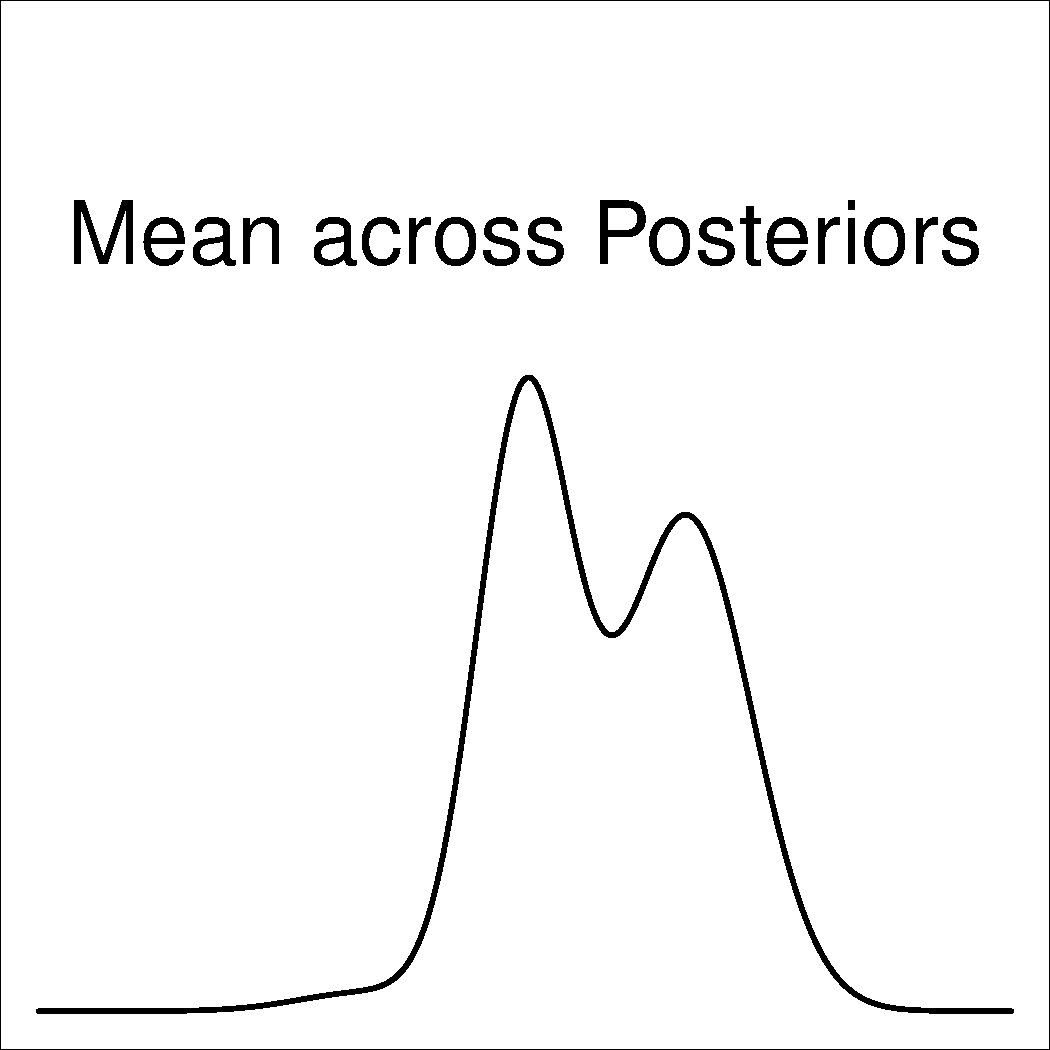
\includegraphics[width=1\textwidth]{bayesian_update_illustration_posterior.pdf}\\
            \end{flushright}
    \end{columns}
\end{frame}

%----------- slide --------------------------------------------------%
\begin{frame}[t]
    \frametitle{Calibrating a single radiocarbon date}
    \begin{flushright}
        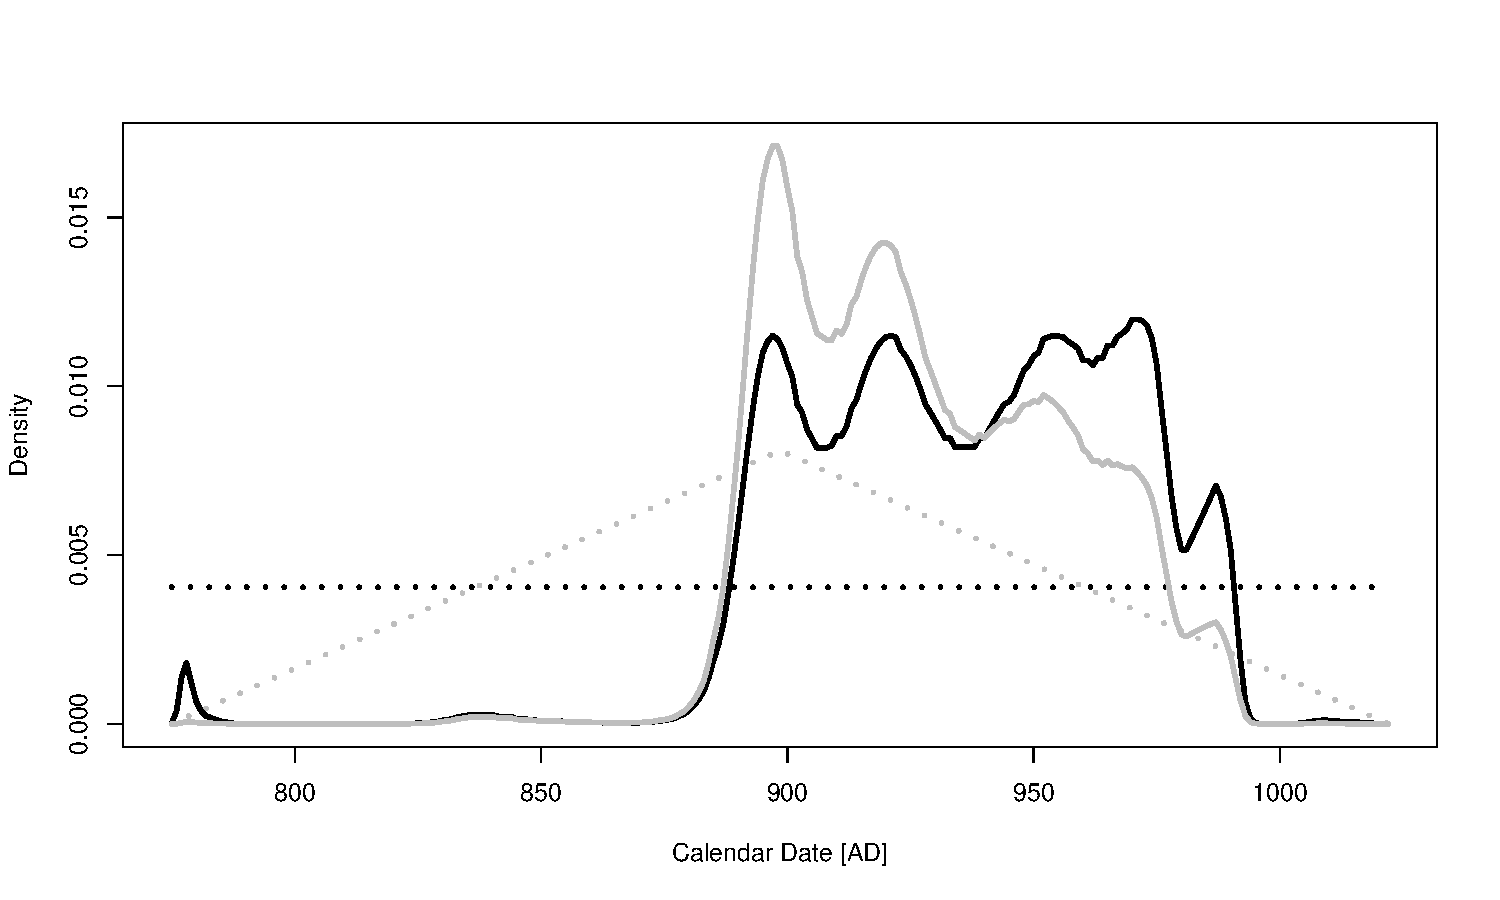
\includegraphics[width=1\textwidth]{single_date_calibration.pdf}\\
    \end{flushright}
\end{frame}

%----------- slide --------------------------------------------------%
\begin{frame}[t]
    \frametitle{On priors and Bayesian radiocarbon}
\end{frame}

%----------- slide --------------------------------------------------%
\begin{frame}[t]
    \frametitle{On MCMC sampling}
\end{frame}

\end{document}